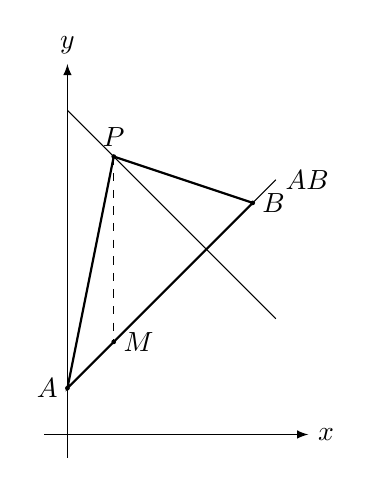
\begin{tikzpicture}[scale=0.5882,>=latex]
  \draw[->] (-0.5,0)--(5.2,0) node[right]{$x$};
  \draw[->] (0,-0.5)--(0,8) node[above]{$y$};
  \draw[domain=0:4.5] plot(\x,{\x+1}) node[right]{$AB$};
  \draw[domain=0:4.5] plot(\x,{-\x+7});
  \coordinate (A) at (0,1);
  \coordinate (B) at (4,5);
  \coordinate (P) at (1,6);
  \coordinate (M) at (1,2);
  \draw[thick] (A)--(B)--(P)--cycle;
  \draw[dashed] (P)--(M);
  \fill (A) circle(1.45pt) node[left]{$A$};
  \fill (B) circle(1.45pt) node[right]{$B$};
  \fill (P) circle(1.45pt) node[above]{$P$};
  \fill (M) circle(1.45pt) node[right]{$M$};
\end{tikzpicture}
